\documentclass[letterpaper]{article}

\usepackage{aaai}
\usepackage{times}
\usepackage{helvet}
\usepackage{courier}
\usepackage{hyperref}
\usepackage{siunitx}
\usepackage{graphicx}
\usepackage{todonotes}
\usepackage{tabularx}
\usepackage{caption}
% \usepackage{placeins}
\sisetup{output-exponent-marker=\ensuremath{\mathrm{e}}}

\frenchspacing
\setlength{\pdfpagewidth}{8.5in}
\setlength{\pdfpageheight}{11in}
\pdfinfo{
    /Title (Email Autoresponder using a Sequence-to-sequence Architecture with BERT)
    /Author (Claudio Scheer, Jose Fernando Possebon Junior)
}
\setcounter{secnumdepth}{0}
\newcommand{\source}[1]{\caption*{Source: {#1}}}
\nocopyright

\begin{document}
% The file aaai.sty is the style file for AAAI Press 
% proceedings, working notes, and technical reports.
%
\title{Email Autoresponder using a Sequence-to-sequence\\Architecture with BERT}
\author{Claudio Scheer \and Jose Fernando Possebon Junior\\
    Pontifical Catholic University of Rio Grande do Sul - PUCRS\\
    \{claudio.scheer, jose.possebon\}@edu.pucrs.br
}

\maketitle

\begin{abstract}
    \begin{quote}
        This paper is related to a practical project of deep learning discipline of Master's in Computer Science of the Pontifical Catholic University of Rio Grande do Sul. We considered that emails are a good source of non-structured data, and that are some automation opportunities. Therefore, we fine-tuned the BERT model to reply emails in the English language. The final model could not be evaluated using a quantitative metric. However, a more subjective metric showed that, in general, the model still presents some problems that allow the human being to recognize when an AI system is replying to an email.
    \end{quote}
\end{abstract}


\section{1. Introduction}

If we consider the scenario of a sales representative who sells software licenses, for example, it is common to receive requests for quotations from their customers about the price of software licenses. There are some opportunities to provide some automation on this task. Therefore, aiming to automate the answering emails task, we implement in this paper an agent that is able to reply an email using a deep learning model.

We can implement this agent with two primary components: one to read the email messages and send the responses and another to receive the email messages parse it and prepare the response based on message content. In this paper, we deal with the piece of software responsible for receiving the message content and generate the proper reply for that message.

A significant amount of software uses Natural Language Understanding (NLU), and they achieve excellent results in understanding the context of messages and generating a proper response to that. Looking for all different approaches that we can use on natural language understanding, dataset availability, and time to implement, we choose to fine-tune a BERT model for the sequence-to-sequence (Seq2Seq) task.

The first idea was to implement something using the Brazilian Portuguese language, and we have looked for some datasets available. We could not find any suitable source of data to train our model. We know that there are many more datasets in the English language available, so we decide to go that way.

We did not implement the piece of checking email inbox and sending the answer email. We consider this task; it is trivial, and it is not the objective of this assignment.

Our goal for this assignment is to provide software capable of receiving any text with some context and producing a meaningful answer to that. To make it happen, we will use a public dataset of emails with responses to train our model and do some experiments. Later on, we will submit a survey to a group of people asking them to identify based on some questions when the answers were from a human or computer software.

In the Section~2, we present some the background about the BERT model and the architecture used in this paper. Section~5 discusses how we parsed the dataset and the results achieved with the fine-tuned model.


\section{2. Background}

For this assignment, we need to understand concepts about language model, sequence-to-sequence (Seq2Seq), attention mechanisms, and transformers. As we saw in classes, when we have a sequence of words, we need to compute the distribution of probabilities of the next word of sequence based on specific vocabulary. This system is known as a language model. Simply we consider language model as a system that defines probabilities to a piece of text. There are some issues with language models based on n-grams: sparse, storage of count of n-grams in memory. Another possibility is to use a trigram approach, but we saw that although the result generated is grammatically complaint on the English language, we do not have a context. So this is not what we need, and we learned too about sequence-to-sequence (Seq2Seq).

\subsection{BERT}

BERT is a short for Bidirectional Encoder Representations from Transformers, proposed by \cite{DBLP:journals/corr/abs-1810-04805}. Transformers network was proposed by \cite{DBLP:journals/corr/VaswaniSPUJGKP17} and use the attention mechanism, proposed by \cite{DBLP:journals/corr/BahdanauCB14}. In a nutshell, the attention mechanism can learn representations between words that express their contextual meaning.

Since BERT is bidirectional, the attention mechanism does not learn only representations of just the previous words, but for all the words in the sentence. To achieve this, BERT was pre-trained for masked language modeling and next sentence predictions tasks. However, with the adjustment of the output layers and a fine-tuning process, the model can be used for other tasks, using the same parameters as the original BERT model.

The original BERT model was pre-trained in a corpus comprising Wikipedia and Book Corpus. Two pre-trained models are available: BERT large, with \num{345}{M} parameters and 24 layers, and BERT base, with \num{110}{M} and 12 layers.

Figure~\ref{fig:transformer} shows the architecture of a Transformer network, proposed by \cite{DBLP:journals/corr/VaswaniSPUJGKP17}. Originally, Transformers was proposed to be used for machine translation tasks, so the architecture has encoder and decoder blocks. BERT uses this same architecture, but trained with different tasks, as previously stated.

The next two sections discusses the BERT model encoder and decoder blocks, used for sequence-to-sequence tasks.

\begin{figure}[ht]
    \centering
    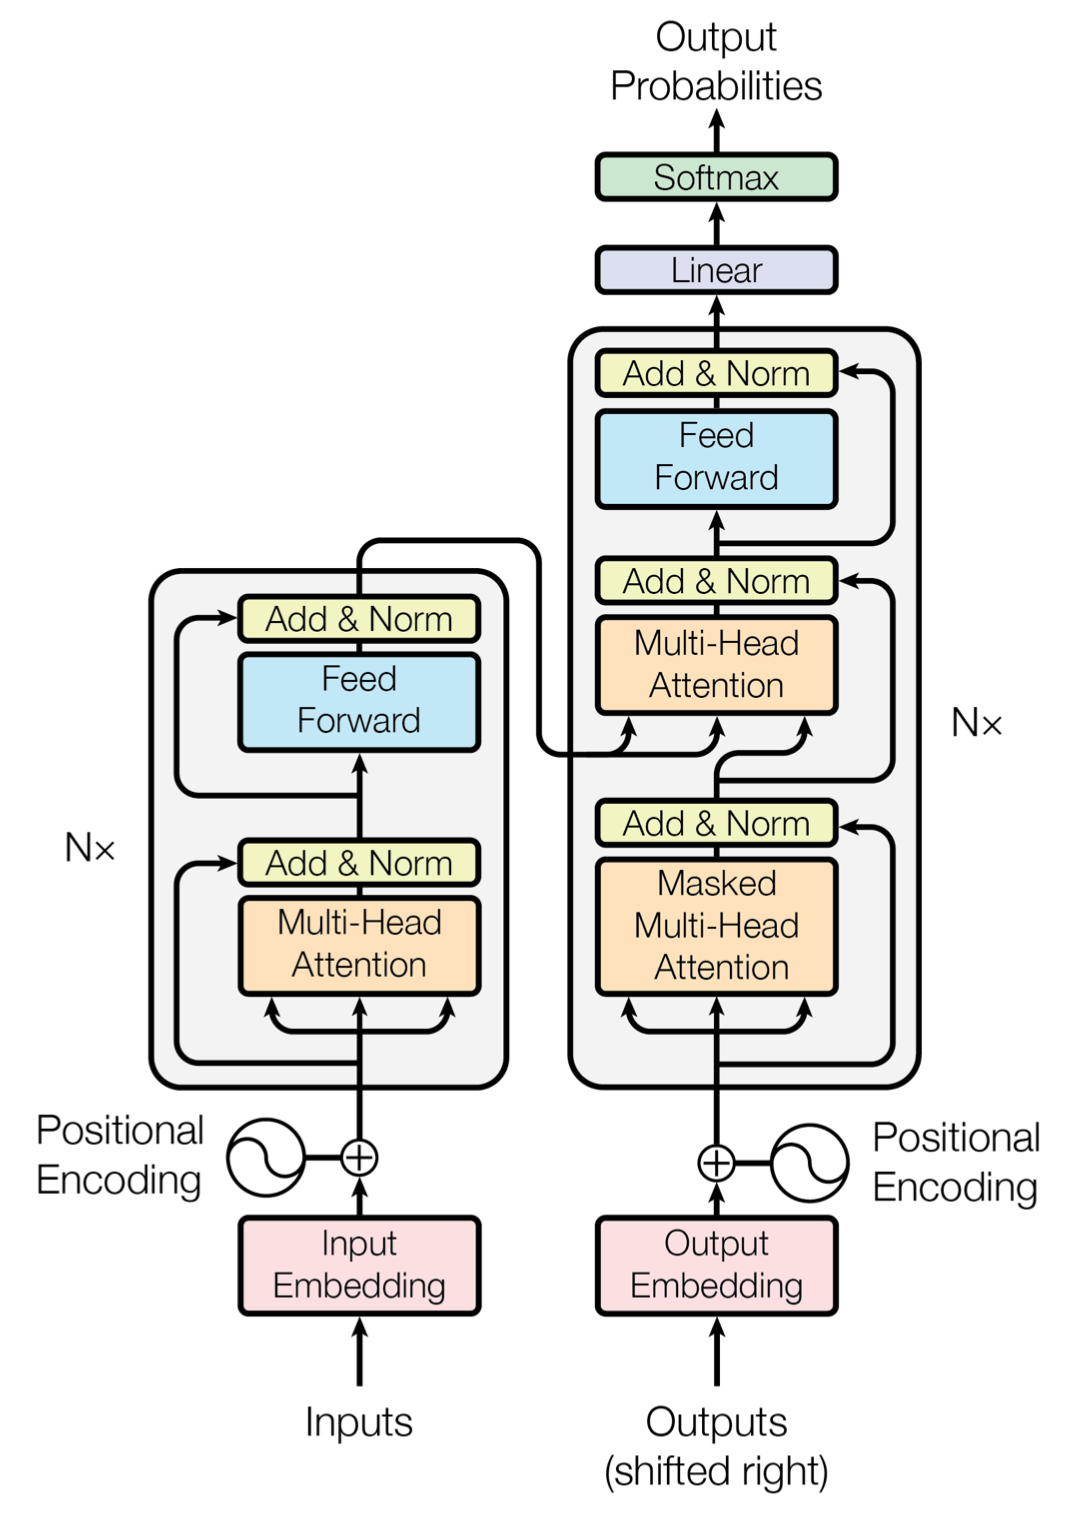
\includegraphics[width=0.47\textwidth]{../images/transformer_architecture.png}
    \caption{Transformer Architecture}
    \label{fig:transformer}
    \source{\cite{DBLP:journals/corr/VaswaniSPUJGKP17}}
\end{figure}

\subsection{BERT encoder}

In the first step, each token in the sequence is embedded in a $N$ dimmensions vector. The position of the token in the sentence is also taken into account. Therefore, after embedding the tokens, positional encoding is added to the embedded matrix. In BERT, the embedding and the position encoding is learned through back-propagation.

The next block in Figure~\ref{fig:transformer} is the encodding block. This block can be chained $n$ times to, intuitively, learn more complex relationships between words. The BERT base architecture chains 12 of these blocks.

\subsection{BERT decoder}

The embedding of the the decoder block is similar to the encoder block. The difference is that the target sentence is shifted with a token to indicate the start and the end of the sentence.

The masked self-attention used in the decoder ignores the words on the right. That is, since the task used in the original Transformer is a language model, the words on the right represents the word that the model needs to learn to predict and should be ignored. This is not true for BERT, as it uses different tasks to train the model.

For BERT, the decoder architecture is almost the same as the encoder architecture. The difference is that, for multi-head attention, the output of the encoder network is used.

% \href{https://medium.com/dissecting-bert/dissecting-bert-part2-335ff2ed9c73}{https://medium.com/dissecting-bert/dissecting-bert-part2-335ff2ed9c73}

% \href{https://medium.com/dissecting-bert/dissecting-bert-part-1-d3c3d495cdb3}{https://medium.com/dissecting-bert/dissecting-bert-part-1-d3c3d495cdb3}

% \href{https://medium.com/dissecting-bert/dissecting-bert-appendix-the-decoder-3b86f66b0e5f}{https://medium.com/dissecting-bert/dissecting-bert-appendix-the-decoder-3b86f66b0e5f}

\section{3. Related work}

We know that there is plenty of work done in this area, so we looked at what others already implemented to have insights and technical information on how to achieve our goal. At first glance, we checked some features implemented by Google on their email service and what theoretical foundations they used. On of the existing features available at Gmail is the Smart Reply that it is an automated response suggestion that users can choose just taping on the suggested text. The concept of Smart Reply is to generate a short reply message looking at the context of the email[cite]. This concept is a good start, but we intend to provide a more detailed answer to our emails. [cite] proposes a different approach to answer generation that it is more aligned with what we intend to achieve. Although the method used seems to be more efficient, we decided to pursue a more straightforward implementation due to our constraints of datasets, computational resources, and time.


\section{4. Experiments and Results}

In this section, we discuss the how the dataset and the implementation of the sequence-to-sequence model was handled and the results achieved.

\subsection{Dataset}

As the project focus is on automatic email reply, The Enron Email Dataset\footnote{\href{https://www.kaggle.com/wcukierski/enron-email-dataset}{https://www.kaggle.com/wcukierski/enron-email-dataset}} was used to train the model. The dataset contains only the emails raw data. Therefore, a parser\footnote{\href{https://www.kaggle.com/claudioscheer/extract-reply-emails}{https://www.kaggle.com/claudioscheer/extract-reply-emails}} was built to extract the email and the replies from the raw data of the email.

To identify whether an email has a reply or not, we look for emails that contain the string \texttt{-----Original Message-----}. After filtering only emails with non-empty replies, those emails were parsed into an input sequence (the original email) and a target sequence (the reply email). The entire extraction was done automatically, that is, we did not extract or adjust any email manually.

Two libraries were used to parse the dataset: \texttt{talon}\footnote{\href{https://github.com/mailgun/talon}{https://github.com/mailgun/talon}}, provided by Mailgun, and \texttt{email}, provided by Python. The \texttt{email} package returns the email body with the entire thread. To extract only the last reply from an email thread, the \texttt{talon} package was used.

The original dataset contains \num{517401} raw emails. After parsing the raw dataset, the new dataset consisted of \num{110205} input and target pairs. As the resources available to fine-tune the model were limited,  only emails with less than \num{256} characters were used. The final dataset consisted of \num{40062} emails. All of these input and target pairs were used to train the BERT model.

\num{21} emails that were not correctly parsed were used to evaluate the model and obtaing the BLEU score. These emails were chosen manually from the dataset.

\subsection{Implementation}

A pre-trained BERT model, provided by Hugging Face\footnote{\href{https://huggingface.co/}{https://huggingface.co/}}, was used. Hugging Face also provides a PyTorch library for using the pre-trained models. Therefore, this library was used to implement the sequence-to-sequence model, with PyTorch 1.5.1.

The \texttt{BertModel} class provided by Hugging Face can behave as an encoder or decoder. The difference is that, for the encoder, only a layer of self-attention is used and, for decoder, a layer of cross-attention is added between the layers of self-attention. The difference between these attention mechanisms is discussed in Section~BERT.

In this paper, the BERT base architecture was used. This model uses fewer resources, which allowed us to increase the batch size. To fine-tune the model, the following hyperparameters was used:

\begin{itemize}
    \item Learning rate: \num{1e-4};
    \item Warm-up steps: \num{5000};
    \item Epochs: \num{10.5};
    \item Adam epsilon: \num{1e-4}, same as in the original BERT paper \cite{DBLP:journals/corr/abs-1810-04805};
    \item Batch size: \num{10};
    \item Beam search hypothesis: \num{3};
\end{itemize}

In the fine-tune process, an EC2 spot instance on AWS was used. A checkpoint of the model was saved every \num{20000} steps, mitigating the loss of processment if the instance was suddenly stopped. The instance was equipped with a NVIDIA T4 GPU (CUDA \num{10.2}), with \num{16}{GB} of memory.

The batch size was limited by the amount of GPU memory available. We also tested to accumulate and update the gradients after \num{4} steps, but we did not see any improvements.

Different values were tested for the learning rate and epochs, with and without warm-up. Figure~\ref{fig:learning-rate-schedule} shows the final results of the learning rate update during the fine-tuning process.

\begin{figure}[ht]
    \centering
    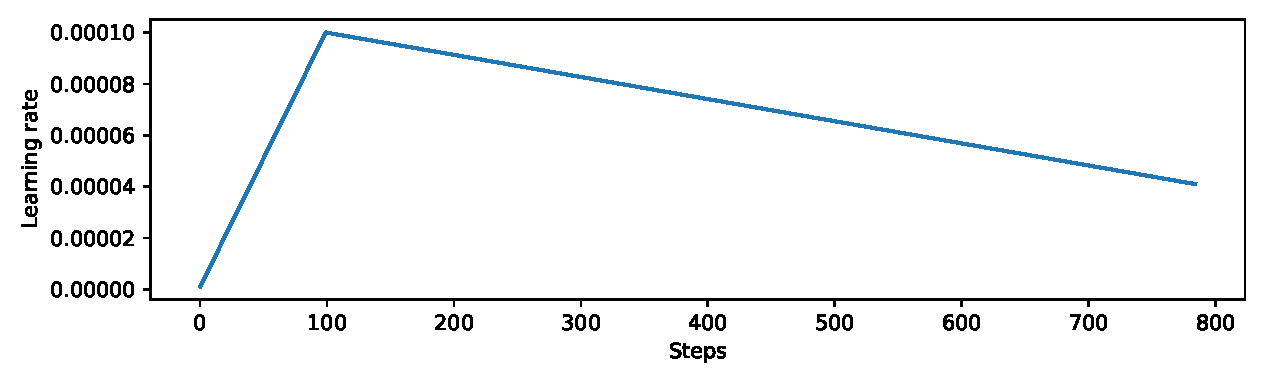
\includegraphics[width=0.47\textwidth]{../images/warmup_linear_schedule.pdf}
    \caption{Learning rate schedule}
    \label{fig:learning-rate-schedule}
\end{figure}

Figure~\ref{fig:loss} shows the loss function value over the fine-tuning process. We do not know why, but loss function shows a greater decrease at the end of each epoch.

\begin{figure}[ht]
    \centering
    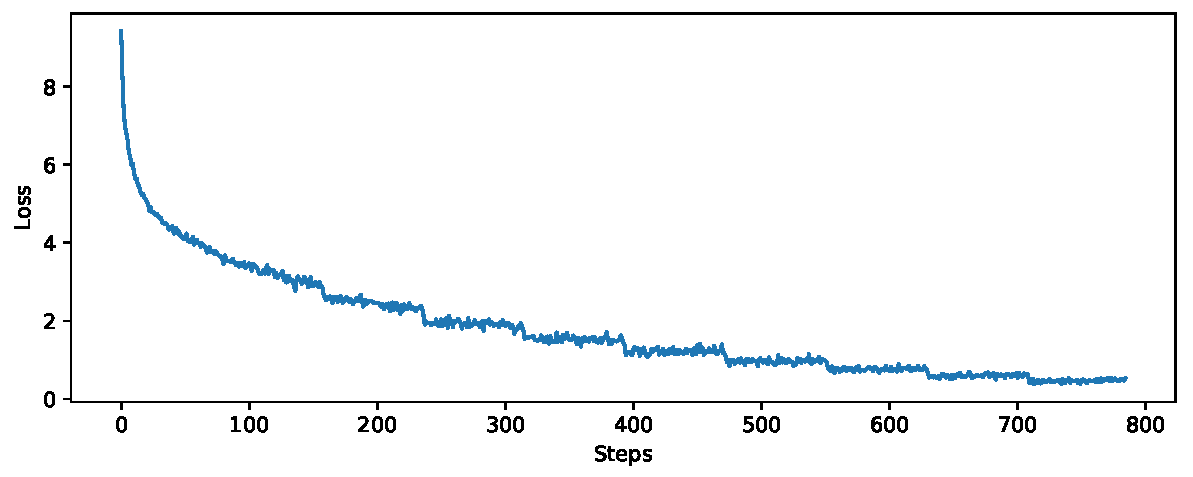
\includegraphics[width=0.47\textwidth]{../images/loss_function.pdf}
    \caption{Loss function}
    \label{fig:loss}
\end{figure}

Some hyperparameters configuration shows bad results in the loss function. For example:

\begin{itemize}
    \item learning rates greater than \num{1e-4} did not make the model converge;
    \item the use of a warm-up period allowed the model to converge in less epochs;
    \item a high number of epochs almost causes an overfitting of the model;
\end{itemize}

The last changed hyperparameter was the number of hypothesis explored in each branch of the beam search. A number greater than \num{3} resulted in more words being out of context in the generated reply email.

\subsection{Results}

% \FloatBarrier
\begin{table*}[ht]
    \centering
    \begin{tabularx}{\textwidth}{|X|X|c|c|}
        \hline
        \textbf{Email} & \textbf{Reply} & \textbf{AI?} & \textbf{Was it AI?} \\
        \hline
        Let me know if this works. & This works great. Will let you know. as soon as I get a chance, let me know & \num{95.7}{\%} & yes \\
        \hline
        Following are the terms under which I ran the Forward Obligation report and received this message: General SQL error. ORA-00907: missing right parenthesis. Terms: Let me know what you find. Thanks! & Kate, I ran the report with the exact same options and it came right up. Try it again, exactly as before. Usually if it works for one person and not the other it is a security issue. Let me know what happens. Thanks, Brettther & \num{52.2}{\%} & yes \\
        \hline
        Didn't you trade uranium at one time? & Yeah, I know the buisness VERY well. & \num{30.4}{\%} & no \\
        \hline
        Are you free for drinks either Monday or Wednesday? & Yes & \num{69.6}{\%} & no \\
        \hline
        Mons, I would be available on the 25th, 26th or 27th. I cannot make it the week of the 18th. Thanks, Bill. & OK, so, let's see if we can get together later today. I have to leave at 16:00 for a few minutes, but I am sure that I will be out at that moment. Thank you Kim. & \num{39.1}{\%} & yes \\
        \hline
    \end{tabularx}
    \caption{Is it AI? test}
    \label{table:is-it-ai-test}
\end{table*}
% \FloatBarrier

The fine-tuned model still has some noise in the replies generated. Therefore, only the first part of the text of the generated replies was used. This is valid for the BLEU score and for the subjective evaluation.

The BLEU score was used to get a quantitative result of the model. Using the evaluation dataset, the BLEU score was \num{0.0}. This does not mean that the replies were bad. This means that the generated replies do not match to the replies originally sent. Table~\ref{table:example-reply-bleu} shows some examples of why the BLEU score was \num{0.0}.

\begin{table}[ht]
    \centering
    \begin{tabularx}{0.47\textwidth}{|X|X|X|}
        \hline
        \textbf{Input} & \textbf{Target} & \textbf{Generated} \\
        \hline
        nevermind.  are you at work? & yea & i'm all alone over here... \\
        \hline
        what re your plans for tomorrow? & drop prentice's car off at shop; go to dome              & leaving early tomorrow. leaving early. leaving early. leaving early. \\
        \hline
        I just refaxed it.  For your information, my total hours is 49. & I noted your hours..I will look for the t/s Thanks Lisa! & Thanks Rick, and let's talk after the holidays about a new game plan... Best regards and happy thanksgiving. Jaime Williams. \\
        \hline
    \end{tabularx}
    \caption{Example of generated replies}
    \label{table:example-reply-bleu}
\end{table}

As shown in Table~\ref{table:example-reply-bleu}, BLEU is not a good option for this problem. Therefore, a subjective assessment of the replies was made. We generated some replies, created a form using Google Forms, and asked some people to answer the questionnaire.

The question asked for each reply generated was: Was this reply generated using Artificial Intelligence software? The interviewee could choose only yes or no. The form contains only five emails and replies. The Table~\ref{table:is-it-ai-test} shows the results of the test answered by 23 human beings. The column `AI?' shows the percentage of answers that believed the reply was generated by an AI system. The column `Was it AI?' shows whether the reply was generated by an AI system or not.

In general, Table~\ref{table:is-it-ai-test} shows that human beings can identify that the reply was generated by an AI system. Also, it is important to note that when the reply is short, most people think that it is generated by an AI system.


\section{5. Final Remarks and Future Work}

Despite the small dataset used and limited resources available, the fine-tuned model performed well. In a further works, the dataset must be revised to avoid data that may cause noise in the predictions. 


\bibliographystyle{aaai}
\bibliography{references}

\end{document}